\def\Module{Principles of Computer System Design}
\def\Uebung{Assignment 2}
\def\Studentenname{Marco Eilers (dbk726)}
\def\Sub_date{13.12.2012}

\documentclass[12pt,a4paper]{article}

\usepackage[utf8]{inputenc}
\usepackage[T1]{fontenc}
\usepackage{fullpage} 
\headsep1cm
\parindent0cm
\usepackage{amssymb, amstext, amsmath}
\usepackage{fancyhdr}
\usepackage{lastpage}
\usepackage{booktabs}
\usepackage{graphicx}
\usepackage{subfigure}
\usepackage{hyperref}
\usepackage{threeparttable}
\usepackage{footnote}
\usepackage{listings}
\usepackage{tikz}
\makesavenoteenv{tabular}

\usetikzlibrary{arrows,automata}

\lhead{\textbf{\Module}}
\rhead{\Uebung~(Submission: \Sub_date)}

\cfoot{}
\lfoot{\Studentenname}
\rfoot{\thepage\ of \pageref{LastPage}}
\pagestyle{fancy}
\renewcommand{\footrulewidth}{0.4pt}

\newcommand{\code}[1]{{\fontfamily{fvm}\small \selectfont #1}}

%Line spacing between paragraphs
\setlength{\parskip}{6pt}

\begin{document}

\title{\Module\\\Uebung}
\author{\Studentenname}
\maketitle

\section*{Exercises} 
\label{sec:exercises}

\subsection*{Question 1}
\label{sec:eq1}

\subsubsection*{(a)}
Schedule 1:
 
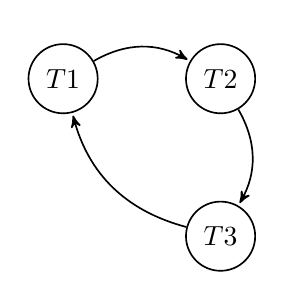
\begin{tikzpicture}[->,>=stealth',shorten >= 1pt,auto,node distance=2.cm,accepting/.style={double distance= 1.5pt},semithick]
\node[state](1) {$T1$};
\node[state] (2) [right of=1] {$T2$};
\node[state] (3) [below of=2] {$T3$};

\path (1) edge [bend left] node {} (2)
      (2) edge [bend left] node {} (3)
      (3) edge [bend left] node {} (1);

\end{tikzpicture}

This schedule is not conflict-serializable, since the precedence graph contains a circle. T1 has to come before T2, which has to come before T3, which has to come before T1, which is impossible.

Schedule 2:

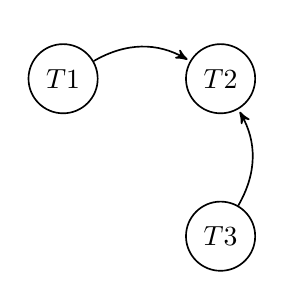
\begin{tikzpicture}[->,>=stealth',shorten >= 1pt,auto,node distance=2.cm,accepting/.style={double distance= 1.5pt},semithick]
\node[state](1) {$T1$};
\node[state] (2) [right of=1] {$T2$};
\node[state] (3) [below of=2] {$T3$};

\path (1) edge [bend left] node {} (2)
      (3) edge [bend right] node {} (2);

\end{tikzpicture}

This one is conflict-serializable, since there is no circle in the precedence graph. A possible serial schedule would be $\text{T1 } \rightarrow\text{ T3 } \rightarrow \text{ T2}$. 

\subsubsection*{(b)}
(Hypothetical) Schedule 1:

\begin{align*}
  \text{T1: } & \text{S(X)} & \text{R(X)} &  & & & & & & & & & & & \text{X(Y)} & \text{W(Y)} & \text{C}\\
  \text{T2: } & & & \text{X(Z)} & \text{W(Z)} & \text{X(X)} & \text{W(X)} & \text{C} & & & & & & & & \\
  \text{T3: } & & & & & & & & &  \text{S(Z)} & \text{R(Z)} & \text{S(Y)} & \text{R(Y)} & \text{C} & & & \\
\end{align*} 

This schedule could not have been generated by Strict 2PL. T1 first gets a shared lock on X. Afterwards, T2 needs a write lock on X. But this would mean that T1 has to commit before T2, which is not the case.

Schedule 2: 

\begin{align*}
  \text{T1: } & \text{S(X)} & \text{R(X)} & & & & & & \text{X(Y)} & \text{W(Y)} & \text{C} & & & & & \\
  \text{T2: } & & & & & \text{S(Z)} & \text{R(Z)} & & & & & \text{X(X)} & \text{W(X)} & \text{X(Y)} & \text{W(Y)} & \text{C} \\
  \text{T3: } & & & \text{X(Z)} & \text{W(Z)} & & & \text{C} & & & & & & & &  
\end{align*}

This one could come from a Strict 2PL scheduler. T1 gets a lock on X and Y before T2 does, and it also commits before T2. Similarly, T3 gets a lock on Z before T2 does, and it also commits before T2. Therefore there are no conflicts, and therefore this schedule does not conflict with Strict 2PL.



\subsection*{Question 2}
\label{sec:eq2}

Scenario 1:
Since T1 has completed before T3 starts, there is no conflict between those two transactions. However, since T2 completes before T3 begins its write phase, we must make sure that WS(T2) $\cap$ RS(T3) is empty. Since both WS(T2) and RS(T3) contain 4, this is not the case, and T3 must be rolled back.

Scenario 2:
Since T1 completes before T3 begins its write phase, we must again make sure that WS(T1) $\cap$ RS(T3) is empty. This is not the case, since both of these sets contain 3. Therefore T3 must be rolled back. In this case it is not important that T2 and T3 actually don't conflict: Since T2 completes its read phase before T3 does, we would have to make sure that WS(T2) $\cap$ RS(T3) and WS(T2) $\cap$ WS(T3) are both empty. This is the case, but as said before, this does not matter, because the conflict between T1 and T3 already forces us to roll back T3.
 
Scenario 3: 
Both T1 and T2 complete before T3 begins its write phase, which means that we must make sure that WS(T1) $\cap$ RS(T3) and WS(T2) $\cap$ RS(T3) are both empty. Since the write sets only contain 4 and 6, respectively, and neither of these elements is in the read set of T3, this is the case, and therefore T3 may commit.


\subsection*{Question 3}
\label{sec:eq3}

(c) In a system that implements Write-Ahead Logging, which are the two situations in which the log
tail must be forced to stable storage? Explain why log forces are necessary in these situations and
argue why they are sufficient for durability.

\subsubsection*{(a)}
Such a system needs neither undo nor redo. Since all commited operations are immediately forced to nonvolatile or even stable storage, no such operations get lost in a crash and therefore we never have to redo them during the recovery process. Similarly, we also know that noncommitted changes only remain in volatile storage and are not written to disk until they are committed. This means that it is impossible for changes to land on disk until it is certain that they will stay there, and therefore we never need to undo any changes.

\subsubsection*{(b)}
The only thing we assume about nonvolatile storage is that the data in it does not automatically get lost during a crash or when the system is intentionally turned off or restarted. That makes it different from volatile storage, which is lost everytime the system is turned off in some way. However, nonvolatile storage may get lost if there are other (mechanical) failures, like a classical disk failure. With stable storage, we assume that this can never ever happen, and that everything that we store in it is guaranteed to remain there without any errors basically forever. In practice, it is nearly impossible to guarantee that, but one can get storage that can be considered "stable" for all practical purposes by using a lot of duplicate nonvolatile storage devices, possibly in different physical locations.

\subsubsection*{(c)}

when committing, all log entries up to lastLSN must be flushed


\subsection*{Question 4}
\label{sec:eq4}

Consider the recovery scenario described in the following, in which we use the
ARIES recovery algorithm. At the beginning of time, there are no transactions active in the system and no
dirty pages. A checkpoint is taken. After that, three transactions, T1, T2, and T3, enter the system and
perform various operations. The detailed log follows:

(a) Apply the ARIES recovery algorithm to the scenario above. Show:
1. the state of the transaction and dirty page tables after the analysis phase;
2. the sets of winner and loser transactions;
3. the values for the LSNs where the redo phase starts and where the undo phase ends;
4. the set of log records that may cause pages to be rewritten during the redo phase;
5. the set of log records undone during the undo phase;
6. the contents of the log after the recovery procedure completes.


\begin{enumerate}
  \item Transaction table: see table \ref{tab:transactions}. Here the entry for T1 has already been removed. The status U denotes transactions that should be undone.
  \item Dirty page table: see table \ref{tab:dirty}.
  \item Losers = $\{T1, T2\}$, Winners = $\{T3\}$
  \item The redo phase starts at LSN 3. The undo phase ends also at LSN 3. 
  \item RewriteRecords = $\{3,4,5,6,8,9\}$
  \item UndoRecords = $\{8,5,4,3\}$
  \item Log after the recovery procedure: see table \ref{tab:after}.
\end{enumerate}

\begin{table}
  \begin{tabular}{c | c | c}
  Transaction ID & Status & lastLSN \\ \hline
  T1 & U & 4\\
  T2 & U & 9 
  \end{tabular}
  \caption{Transaction table after the analysis phase}
  \label{tab:transactions}
\end{table}

\begin{table}
  \begin{tabular}{c|c}
  Page & recLSN \\ \hline
  P2 & 3 \\
  P1 & 4 \\
  P5 & 5 \\
  P3 & 6 
  \end{tabular}
  \caption{Dirty page table after the analysis phase}
  \label{tab:dirty}
\end{table}

\begin{table}
  \begin{tabular}{l | l | l | l | l}
  LSN & LAST\_LSN & TRAN\_ID & TYPE & PAGE\_ID \\ \hline
  1 & - & - & begin CKPT & - \\
  2 & - & - & end CKPT & - \\
  3 & NULL & T1 & update & P2 \\
  4 & 3 & T1 & update & P1 \\
  5 & NULL & T2 & update & P5 \\
  6 & NULL & T3 & update & P3 \\
  7 & 6 & T3 & commit & - \\
  8 & 5 & T2 & update & P5 \\
  9 & 8 T2 & update & P3 \\
  10 & 6 & T3 & end & - 
    
  \end{tabular}
  \caption{The log after the recovery procedure completes}
  \label{tab:after}
\end{table}


\section*{Programming} 
\label{sec:programming}

\subsection*{Question 1}
\label{sec:pq1}

Both Logger and Checkpointer are threads that are started once at the beginning and continue to run as long as the web service is available. The Logger has a queue of log requests, which consist of a LogRecord and a Future. For each call of \texttt{logRequest}, a new Future is created. This future, along with the incoming LogRecord, is then put in said queue and the Future is returned immediately. The Logger thread polls the queue in an endless loop, and for every pair of LogRecord and Future it first writes (and forces) the LogRecord to disk (by simply serializing the LogRecord object) and then sets the Future's status to done. Any methods that manipulate the database therefore have to call logRequest and then wait until the returned Future's state is changed to done.

The Checkpointer is also a thread running in an endless loop. It waits for a certain amount of time and then calls \texttt{quiesce} on KeyValueBaseLogImpl, another object that is created only once at the beginning. Quiesce is implemented via a MasterLock, another ReentrantReadWriteLock. All other operations now request a shared ("read") lock from this central component before they do anything else and return the lock when everything is done, which means that those operations can still run concurrently. \texttt{quiesce}, however, requests an exclusive ("write") lock, which means that as soon as this lock is acquired, all other operations can no longer get their read lock and have to wait. It is guaranteed that the function will get its write lock at some point (although it may take a while), since I use the fair scheduler. \texttt{resume} then simply releases the write lock again. Between those two function calls, the Checkpointer flushes the Store, writes the current Index to disk and truncates the log. If the key-value-store is currently initialized, it will also write an empty init operation (meaning a call to init that does not point to an initialization file) in the new log, so that during recovery the store knows whether it has already been initialized.

When the server is started and it detects that a log file is present, it first deserializes the Index, updates it to use the MemoryMappedFile that is on disk, and then steps through the log file and re-invokes every method call that is recorded in it. A flag is set before this, so that REDOing these operations is not logged again.


\subsection*{Question 2}
\label{sec:pq2}
Describe how you tested your implementation of both components and ensured that
durability was actually achieved in face of fail-stop failures. (2 paragraphs)


\subsection*{Question 4}
\label{sec:pq4}
Explain how you can quantify the overhead of log-based durability in both throughput and
latency. Design and describe your experimental setup to quantify this overhead. Recall that you must
document all parameters that may influence the performance of the system (e.g., e.g., number of clients,
hardware characteristics, size of dataset managed, mix of operations).


\subsection*{Question 5}
\label{sec:pq5}
Carry out the experiment you described in Question 4 and report your overhead results.
Explain the effects you observe regarding throughput and latency of your service.


\subsection*{Question 6}
\label{sec:pq6}

Briefly describe how you implemented group commit in KeyValueBase. (1 paragraph)



 
\begin{thebibliography}{1}


\end{thebibliography}



\end{document}
